\chapter{AODV}
    Ad-hoc On-demand Distance Vector (\aodv) est un protocole réactif à vecteur de distance.
    Les 3 types de messages définis dans \aodv\ sont les Route requests (\textit{\rreq s}),
    les Route Remplies (\textit{\rrep s}) et les Route Errors (\textit{\rerr s}).
    Comme illustré sur la figure suivante, le premier sera envoyé en flooding par un noeud
    désirant obtenir une nouvelle route pour
    une desination donnée. Le second sert de réponse au premier. Il est envoyé à l'émetteur du
    \rreq. Et le dernier sert notamment lorsqu'un lien d'une route active est brisé. 
    Nous détaillons plus bas ces mécanismes.
    \vspace{1cm}
    \begin{figure}[H]
        \centering
        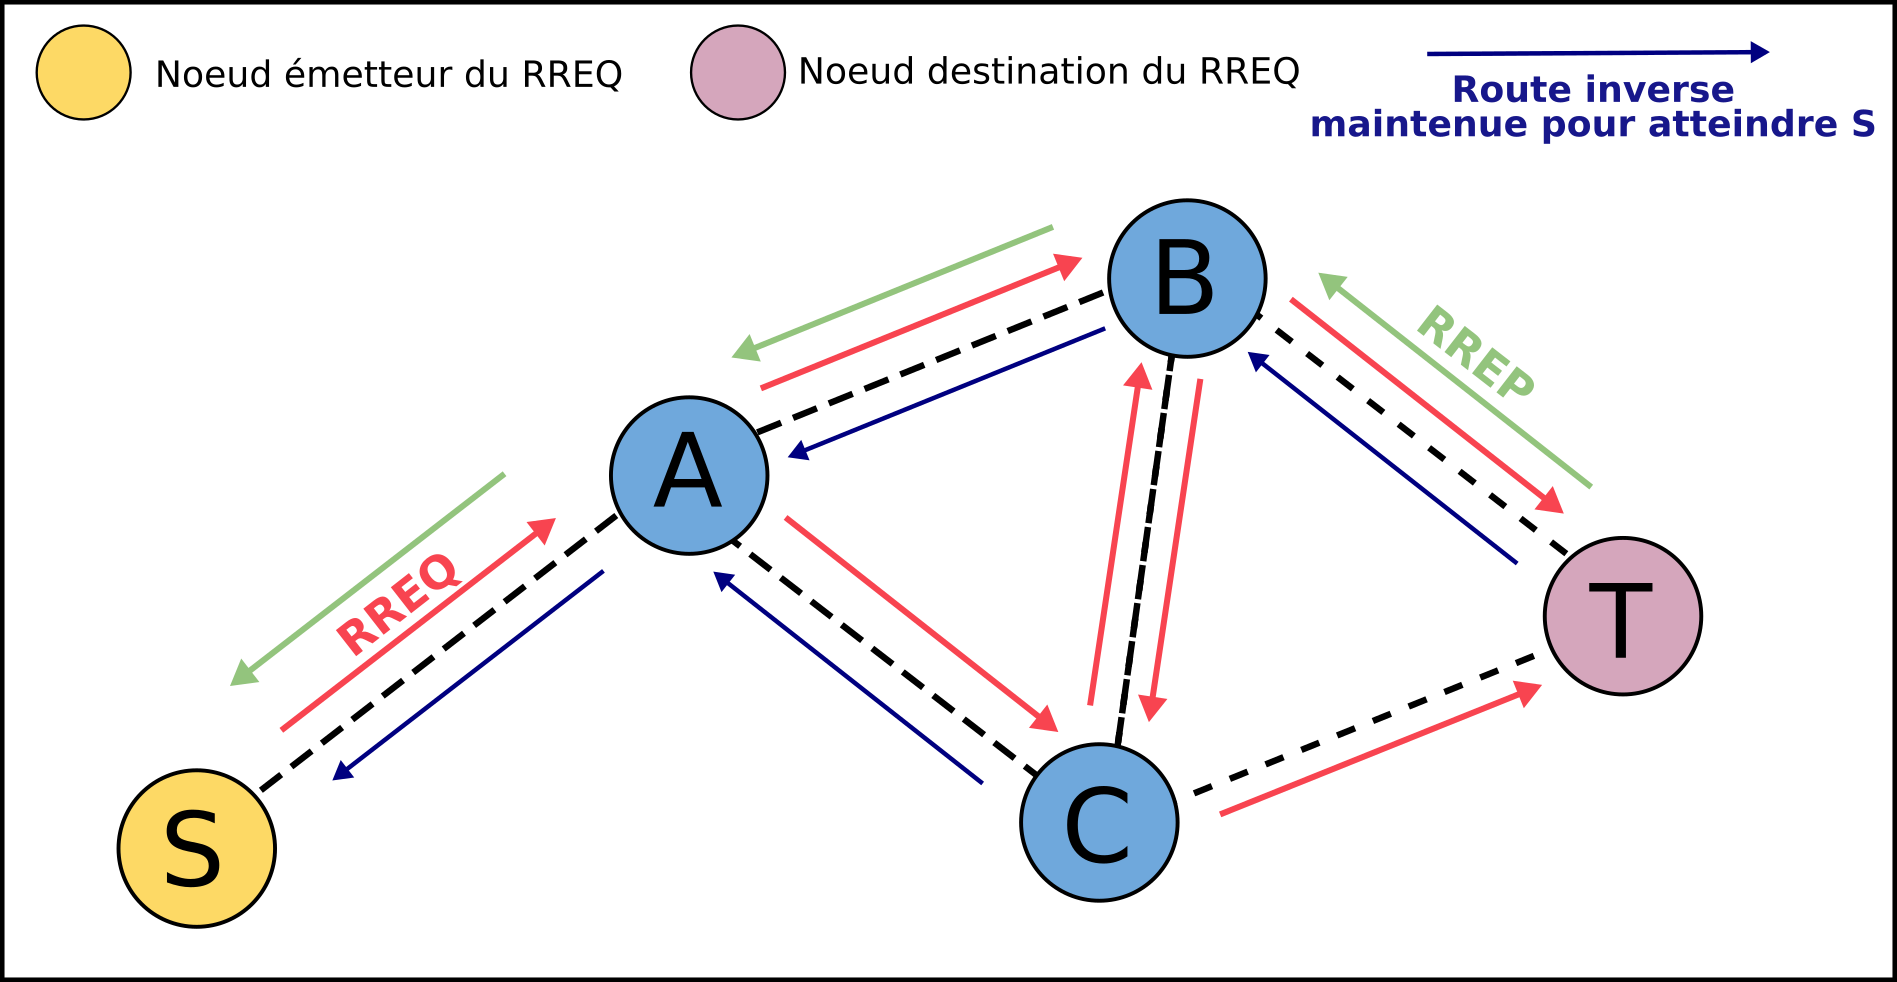
\includegraphics[scale=0.35]{images/aodv.png}
        \caption{Illusration du fonctionnement d'AODV}
        \label{aodv}
    \end{figure}
    
    
    \vspace{0.5cm}
    %\textbf{Format des paquets}\\
    \section{Format des paquets}
        \textbf{RREQ}\\
            \begin{figure}[H]
                \centering
                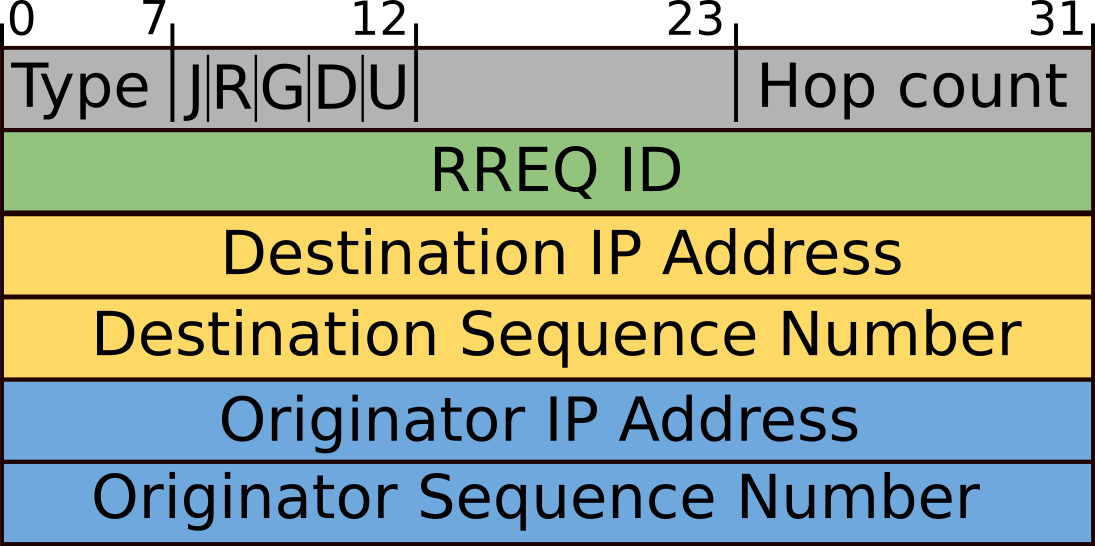
\includegraphics[scale=0.5]{images/rreq.png}
                \caption{Format d'un paquet \rreq\ \cite{rfc_aodv}}
                \label{rreqPaquet}
            \end{figure}
            Le format d'un \rreq\ est illustré sur la figure précédente. Il contient les champs
            repris dans la table suivante:\\
            \begin{table}[H]
                \begin{tabular}{ll}
                    type & \makecell[l]{$=1$}\\\hline
                    J R G & \makecell[l]{flags}\\\hline
                    D  & \makecell[l]{flag indiquant que seul la destination peut\\ répondre au \rreq}\\\hline
                    U & \makecell[l]{flag indiquant que le numéro de séquence de la\\ destination est inconnu}\\\hline
                    Hop count & \makecell[l]{nombre de sauts depuis le noeud source}\\\hline
                    \rreq\ \textsc{id} & \makecell[l]{numéro de séquence identifiant le \rreq}\\\hline
                    Destination IP Address & \makecell[l]{adresse \textsc{ip} du noeud pour lequel la route\\ est demandée}\\\hline
                    Destination Sequence Number & \makecell[l]{le dernier numéro de séquence connu pour une \\route vers la destination}\\\hline
                    Originator IP Address & \makecell[l]{adresse ip de l'émetteur du \rreq}\\\hline
                    Originator Sequence Number & \makecell[l]{numéro de séquence à utiliser pour une route\\ pointant vers l'émetteur du \rreq}\\
                \end{tabular}
                \caption{Champs d'un \rreq\ \cite{rfc_aodv}}
                \label{rreq_fields}
            \end{table}
            
        \textbf{RREP}\\
            \begin{figure}[H]
                \centering
                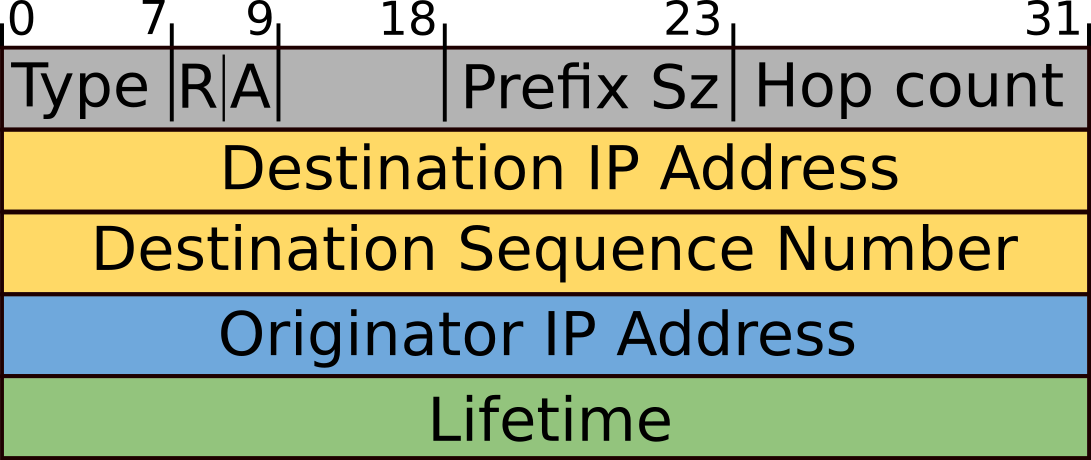
\includegraphics[scale=0.5]{images/rrep.png}
                \caption{Format d'un \rrep\ \cite{rfc_aodv}}
                \label{rreqPaquet}
            \end{figure}
            Le format d'un \rrep\ est illustré sur la figure précédente. Il contient les champs
            repris dans la table suivante:\\
            \begin{table}[H]
                \begin{tabular}{ll}
                    type & \makecell[l]{$=2$}\\ \hline
                    R & \makecell[l]{flag utilisé pour le multicast}\\ \hline
                    Prefix size & \makecell[l]{utilisé pour les aggrégations de routes}\\ \hline
                    Hop Count & \makecell[l]{nombre de sauts de l'\textit{originator} à la destination}\\ \hline
                    Destination IP address & \makecell[l]{adresse IP de du noeud pour qui l'adresse \\est demandée}\\ \hline
                    Destination Sequence Number & \makecell[l]{numéro de séquence de destination \\associé à la route}\\ \hline
                    Originator IP address & \makecell[l]{adresse IP du noeud émetteur du \rreq}\\ \hline
                    Lifetime & \makecell[l]{temps (en ms) pendant lequel le noeud qui reçoit \\le \rrep\ va considérer la route valide}\\
                \end{tabular}
                \caption{Champs d'un \rrep\ \cite{rfc_aodv}}
                \label{rrep_fields}
            \end{table}

    %\textbf{Découverte d'un chemin}\\
    \section{Découverte d'un chemin}
        La découverte d'un chemin est intiée par un noeud voulant envoyer des paquets à une destination pour laquelle il n'a aucune route valide.
        Chaque noeud possède deux compteurs: \textit{sequence\_number} et \textit{rreq\_id}.
        
        
        \vspace{0.5cm}
        \textbf{Génération du RREQ}\\
            Le noeud source incrémente ses compteurs \textit{sequence\_number} et \textit{rreq\_id} de 1.
            Il envoie ensuite un \rreq\ en broadcast à ses voisins.
        
        
        \vspace{0.5cm}
        \textbf{Propagation du RREQ}\\
            \begin{itemize}
                \item[$\bullet$] Noeud intermédiaire\\
                    A la réception d'un \rreq, un noeud intermédiaire va pouvoir rajouter ou mettre à jour
                    les routes vers son prédécesseur et vers le noeud source du \rreq.\\
                    Ensuite deux situations sont possibles:
                    \begin{enumerate}
                        \item Le noeud courant possède une route active vers la destination et le numéro de séquence de la route est plus grand 
                            ou égal au numéro de séquence de la destination dans le \rreq.
                            Dans ce cas, il peut envoyer par unicast un \rrep\ à la source du \rreq.
                        \item Sinon\\
                            Le noeud va incrémenter le nombre de sauts du \rreq\ et le propager à ses voisins.
                    \end{enumerate}

                \item[$\bullet$] Noeud destination\\
                    A la réception d'un \rreq\  lui étant destiné, un noeud va, comme un noeud intermédiaire, 
                    rajouter ou mettre à jour les routes vers son prédécesseur et vers le noeud source du \rreq.
                    Si le \textit{Destination Sequence Number} du \rreq\ est égal à son \textit{sequence\_number},
                    il va incrémenter ce dernier et envoyer un \rrep\ en unicast vers la source du \rreq.     
            \end{itemize}

        \vspace{0.5cm}
        \textbf{Propagation du RREP}\\
            A la réception d'un \rrep\ , un noeud va pouvoir rajouter ou mettre à jour
            les routes vers le noeud source du \rrep\  et vers son successeur.\\
            Il va ensuite incrémenter le nombre de sauts du \rrep\  et le propager en unicast vers la destination de ce \rrep\ .
            Cette propagation en unicast vers la source du \rreq\ est possible par l'apprentissage de la route inverse
            (destination du \rreq\ vers l'émetteur du \rreq) réalisée lors du flooding du \rreq.

    %\underline{\textbf{Table de routage}}\\
    \section{Table de routage}
        Chaque entrée d'une table de routage contient les informations suivantes:
        
        \begin{table}[H]
            \centering
            \begin{tabular}{|l|l|}
                \hline
                \textit{dest}       & Adresse IP de destination\\
                \textit{dest\_SN}   & Numéro de séquence de destination\\
                \textit{flag}       & Indicateur de numéro de séquence de destination valide\\
                \textit{out}        & Interface réseau\\
                \textit{hops}       & \makecell[l]{Comptage de sauts (nombre de sauts nécessaires\\ pour atteindre la destination)}\\
                \textit{next-hop}   & Prochain saut\\
                \textit{precursors} & Liste des précurseurs\\
                \textit{lifetime}   & temps d'expiration ou de suppression de l'itinéraire\\
                \hline
            \end{tabular}
            \caption{entrée d'une table de routage \aodv \cite{rfc_aodv}}
            \label{routingTable_aodv}
        \end{table}

        \textbf{Mise à jour de la table de routage}\\
            Soit N une nouvelle route et O la route existante.\\
            O est mise à jour si:\\
            \begin{center}
                \begin{tabular}{|l|}
                    \hline
                    $O.SN \leq N.SN$ \\
                    \textbf{ou} ($O.SN = N.SN$ \textbf{et} $O.hop\_count > N.hop\_count$)\\
                    \hline
                \end{tabular}
            \end{center}
        
        \textbf{Gestion du \textit{lifetime}}\\
            Le temps de vie d'une route dans la table de routage est initialisé à \textit{active\_route\_timeout} (3 millisecondes).\\
            Quand ce timer expire, la route passe de active à inactive. Une route inactive ne pourra plus être utilisée pour transférer des données
            mais pourra fournir des informations pour de futurs \rreq\  et la réparation de routes.\\
            Quand une route est utilisée, son temps de vie  est actualisé à: $current time + active\_route\_timeout$

    %\vspace{0.5cm}
    %\textbf{Evitement de boucles}\\
    \section{Evitement de boucles}
        A priori les numéros de séquences suffisent pour éviter les boucles. Cependant, d'après \cite{loop_aodv}, il y a des
        ambiguités dans le RFC \cite{rfc_aodv}. Dû à ces ambiguités, l'implémentation pourrait introduire des boucles.
        %Certaines parties du RFC concerant la gestion des numéros de séquences pourraient introduiredes boucles. 
        Nous approfondirons la lecture de cet article si nous choisissons ce protocole afin d'éviter les boucles dans notre implémentation.

        %\vspace{0.5cm}
    %\textbf{Défaillance d'un lien}\\
    \section{Défaillance d'un lien}
        Un noeud faisant partie d'une route active broadcast des messages \textit{hello} (\rrep)
        régulièrement.\\
        Si un noeud ne reçoit pas de message durant un certain temps pour un voisin, il va considérer
        que le lien avec ce voisin est perdu.\\
        Dans ce cas, il va en informé ses voisins impactés par un \textsc{rerr}.
    
    \section{Discussion}
        Ce protocole semble plus robuste que \espmesh. Car en comparaison avec ce dernier, si un noeud tombe,
        les noeuds peuvent trouver une autre route pour envoyer des pauqtes d'un point à un autre.
        A priori cette robustesse dépend également de certains paramètre comme le temps de vie ou la fréquence
        d'émission des messages \textit{hello}.
        